%% ==============================================================
%% DIRECT ACYCLIC GRAPH
%% ==============================================================

\begin{figure}[t]
\centering
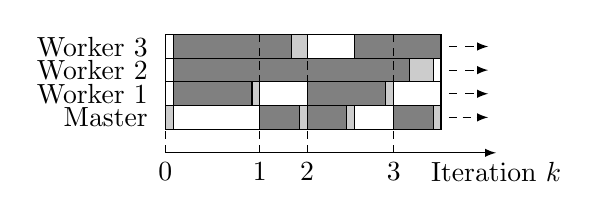
\begin{tikzpicture}
% Worker 1
\draw[black] (0,0.4) rectangle (0.1,0.7);
\draw[black,fill=gray!100](0.1,0.4) rectangle (1.1,0.7); % cd = 2, td = 0.1
\draw[black,fill=gray!40] (1.1,0.4) rectangle (1.2,0.7);
\draw[black] (1.2,0.4) rectangle (1.8,0.7);
\draw[black,fill=gray!100](1.8,0.4) rectangle (2.8,0.7);
\draw[black,fill=gray!40](2.8,0.4) rectangle (2.9,0.7);
\draw[black] (2.9,0.4) rectangle (3.5,0.7);
\draw[dashed,->,>=latex] (3.6,0.55) -- (4.1,0.55); 

% Worker 2
\draw[black](0,0.7) rectangle (0.1,1);
\draw[black,fill=gray!100](0.1,0.7) rectangle (3.1,1); % cd = 3, td = 0.3
\draw[black,fill=gray!40] (3.1,0.7) rectangle (3.4,1);
\draw[black](3.4,0.7) rectangle (3.5,1);
\draw[dashed,->,>=latex] (3.6,0.85) -- (4.1,0.85); 

% Worker 3
\draw[black](0,1) rectangle (0.1,1.3);
\draw[black,fill=gray!100](0.1,1) rectangle (1.6,1.3); % cd = 1.5, td = 0.2
\draw[black,fill=gray!40] (1.6,1) rectangle (1.8,1.3);
\draw[black] (1.8,1) rectangle (2.4,1.3);
\draw[black,fill=gray!100](2.4,1) rectangle (3.5,1.3);
\draw[dashed,->,>=latex] (3.6,1.15) -- (4.1,1.15); 

% Master
\draw[black,fill=gray!40] (0,0.1) rectangle (0.1,0.4); % cd = 0.5, td = 0.1
\draw[black] (0.1,0.1) rectangle (1.2,0.4);
\draw[black,fill=gray!100] (1.2,0.1) rectangle (1.7,0.4);
\draw[black,fill=gray!40] (1.7,0.1) rectangle (1.8,0.4);
\draw[black,fill=gray!100] (1.8,0.1) rectangle (2.3,0.4);
\draw[black,fill=gray!40] (2.3,0.1) rectangle (2.4,0.4);
\draw[black] (2.4,0.1) rectangle (2.9,0.4);
\draw[black,fill=gray!100] (2.9,0.1) rectangle (3.4,0.4);
\draw[black,fill=gray!40] (3.4,0.1) rectangle (3.5,0.4);
\draw[densely dashed,->,>=latex] (3.6,0.25) -- (4.1,0.25); 

% Axis
\node[below] (k1)  at (1.2,-0.2) {$1$};
\node[below] (k2) at (1.8,-0.2) {$2$};
\node[below] (k3) at (2.9,-0.2) {$3$};
\draw[->,>=latex] (0,-0.2) -- (4.2,-0.2) node[below]{Iteration $k$} ;

% Vertical lines
\draw[densely dashed] (0,-0.2) -- (0,1.3);
\draw[densely dashed] (1.2,-0.2) -- (1.2,1.3);  
\draw[densely dashed] (1.8,-0.2) -- (1.8,1.3);  
\draw[densely dashed] (2.9,-0.2) -- (2.9,1.3);    

% Names
\node[below] (axis) at (0,-0.2) {$0$};
\node[left] (M)  at (-0.1,0.25) {Master};
\node[left] (W1) at (-0.1,0.55) {Worker 1};
\node[left] (W2) at (-0.1,0.85) {Worker 2};
\node[left] (W3) at (-0.1,1.15) {Worker 3};

%\node[data] (Y) at (0,0) {$\Yb$};
%% Left part
%\node (M) at (-4,2) {$\M$};
%\node[hp] (xi) at (-4,3) {$\xi$};
%%%
%\node (dM) at (-2,1) {$\dMb$};
%\node[hp] (nu) at (-1.5,2) {$\nu$};
%\node (Psi) at (-2.5,2) {$\bPsi$};
%\node[hp] (apsi) at (-3,3) {$\apsi$};
%\node[hp] (bpsi) at (-2,3) {$\bpsi$};
%%%
%% Middle part
%\node (Sig) at (0,1) {$\sig$};
%\node[hp] (asig) at (-0.5,2) {$\asig$};
%\node[hp] (bsig) at (0.5,2) {$\bsig$};
%%%
%% Right part
%\node (A) at (2,1) {$\Ab$};
%\node[hp] (eps) at (1.5,2) {$\eps$};
%\node (X) at (2.5,2) {$\Xb$};
%\node (Z) at (2,3) {$\Z$};
%\node (s) at (3,3) {$\s$};
%\node (beta) at (1.5,4) {$\mathbf{\bbeta}$};
%\node[hp] (as) at (2.5,4) {$\as$};
%\node[hp] (bs) at (3.5,4) {$\bs$};
%%%
%
%%%
%% Link (chemin en étoile)
%\draw[<-,>=latex] (Y) edge[out=180, in=-75] (dM)
%                      edge (Sig); % [bend right]
%\draw[<-,>=latex] (Y.east) to[out=0, in=225] (A);                      
%%
%\draw[<-,>=latex] (A) edge (X)
%                      edge (eps);
%\draw[<-,>=latex] (X) edge (Z)
%                      edge (s);
%\draw[->,>=latex] (beta) to[bend left] (Z);                                           
%%
%\draw[<-,>=latex] (Sig) edge (asig)
%                        edge (bsig);
%%                                          
%\draw[<-,>=latex] (s) edge (as)
%                      edge (bs);
%%                   
%\draw[<-,>=latex] (dM) edge (Psi)
%                       edge (nu);                     
%\draw[<-,>=latex] (Psi) edge (apsi)
%                        edge (bpsi);
%%                     
%\draw[->,>=latex] (M) to[in=180,out=-75] (dM);
%\draw[->,>=latex] (xi) -- (M);
\end{tikzpicture}
\caption{Illustration of an asynchronous distributed mechanism (idle time in white, transmission delay in light gray, computation delay in gray). The master node is triggered whenever it has received information from $\nmworker$ workers ($\nmworker~=~1$ in the illustration).}
\label{fig:async}
\end{figure}
